\section{Results}
\label{sec:results}

% We present results in two parts:
Our results are twofold:
\begin{enumerate*}
\item main evaluation three Skills conditions across 7 LLM--agent combinations on 84 tasks, and
\item detailed analysis of Skills design factors including quantity, complexity, and domain effects.
\end{enumerate*}
%==============================================================================
\subsection{Experiment 1: Skills Efficacy Across LLM--Agent Combinations}
%==============================================================================

We evaluate how curated and self-generated Skills affect agent performance across commercial model-harness configurations.
We test each configuration under three conditions on all 84 tasks: no Skills, with curated Skills, and with self-generated Skills (where supported).

\subsubsection{Main Results}

\autoref{tab:main-results} presents pass rates across all three conditions for each model-harness combination, ordered by with-Skills performance.

% \begin{table}[t]
% \centering
% \small
% \caption{Pass rates (\%) comparing no-Skills vs.\ with-Skills conditions across 85 tasks. $\Delta$ = improvement. Configurations ordered by overall pass rate. Exception rate shows proportion of runs failing due to harness errors.}
% \label{tab:main-results}
% \begin{tabular}{llcccc}
% \toprule
% \textbf{Harness} & \textbf{Model} & \textbf{No Skills} & \textbf{With Skills} & \textbf{$\Delta$} & \textbf{Exc.} \\
% \midrule
% Codex & GPT-5.2 & 41.8 & 49.5 & +7.7 & 3.4\% \\
% Claude Code & Opus 4.5 & 23.6 & 43.0 & +19.3 & 5.0\% \\
% Gemini CLI & Gemini 3 Flash & 30.9 & 40.1 & +9.2 & 8.9\% \\
% Gemini CLI & Gemini 3 Pro & 23.4 & 37.8 & +14.3 & 8.1\% \\
% Terminus-2 & Gemini 3 Flash & 23.2 & 32.9 & +9.8 & 14.0\% \\
% T2-Skills & Opus 4.5 & 13.8 & 34.5 & +20.7 & 56.3\% \\
% T2-Skills & Gemini 3 Pro & 20.8 & 29.9 & +9.1 & 31.7\% \\
% Terminus-2 & Gemini 3 Pro & 21.3 & 28.9 & +7.7 & 9.8\% \\
% Claude Code & Sonnet 4.5 & 12.5 & 27.2 & +14.7 & 5.9\% \\
% T2-Skills & Gemini 3 Flash & 7.4 & 34.3 & +26.9 & 41.3\% \\
% T2-Skills & GPT-5.2 & 13.3 & 28.8 & +15.5 & 44.7\% \\
% Claude Code & Haiku 4.5 & 5.4 & 25.2 & +19.9 & 2.0\% \\
% T2-Skills & Haiku 4.5 & 10.7 & 24.6 & +13.9 & 59.8\% \\
% T2-Skills & Sonnet 4.5 & 3.5 & 28.1 & +24.6 & 65.3\% \\
% \midrule
% \textbf{Mean} & & 18.0 & 32.4 & +14.4 & -- \\
% \bottomrule
% \end{tabular}
% \end{table}

% \begin{table}[t]
% \centering
% \small
% % \caption{Pass rates (\%) across three Skills conditions on 84 tasks (Method D scoring). $\Delta_\text{S}$ = curated Skills improvement over no Skills. Self-Gen = self-generated Skills; $\Delta_\text{G}$ = self-generated improvement over no Skills. Configurations ordered by with-Skills pass rate. ``--'' indicates condition not evaluated.}
% \caption{Pass rates (\%) across three Skills conditions on 84 tasks. $\Delta_\text{abs}$ = absolute improvement (pp) of curated Skills over no Skills. Self-Gen = self-generated Skills; $\Delta_\text{G}$ = self-generated improvement (pp) over no Skills. Configurations ordered by with-Skills pass rate. ``--'' indicates condition not evaluated.}
% \label{tab:main-results}

% \resizebox{\columnwidth}{!}{%
% \begin{tabular}{llccccc}
% \toprule
% \textbf{Harness} & \textbf{Model} & \textbf{No Skills} & \textbf{With Skills} & \textbf{$\Delta_\text{S}$} & \textbf{Self-Gen} & \textbf{$\Delta_\text{G}$} \\
% \midrule
% Gemini CLI & Gemini 3 Flash & 31.3 & 48.7 & +17.4 & -- & -- \\
% Claude Code & Opus 4.5 & 22.0 & 45.3 & +23.3 & 21.6 & --0.4 \\
% Codex & GPT-5.2 & 30.6 & 44.7 & +14.1 & 25.0 & --5.6 \\
% Claude Code & Opus 4.6 & 30.6 & 44.5 & +13.9 & 32.0 & +1.4 \\
% Gemini CLI & Gemini 3 Pro & 27.6 & 41.2 & +13.6 & -- & -- \\
% Claude Code & Sonnet 4.5 & 17.3 & 31.8 & +14.5 & 15.2 & --2.1 \\
% Claude Code & Haiku 4.5 & 11.0 & 27.7 & +16.7 & 11.0 & 0.0 \\
% \midrule
% \textbf{Mean} & & 24.3 & 40.6 & +16.2 & 21.0 & --1.3 \\
% \bottomrule
% \end{tabular}%
% }
% \end{table}

\begin{table}[t]
\centering
\small
\caption{Pass rates (\%) and normalized gain ($g$) across three Skills conditions on 84 tasks. $g$ measures proportional improvement toward perfect performance (\autoref{eq:normalized_gain}). Configurations ordered by with-Skills pass rate. ``--'' indicates condition not evaluated.}
\label{tab:main-results}
\resizebox{\columnwidth}{!}{%
\begin{tabular}{llccccc}
\toprule
& & & \multicolumn{2}{c}{\textbf{Curated Skills}} & \multicolumn{2}{c}{\textbf{Self-Generated}} \\
\cmidrule(lr){4-5} \cmidrule(lr){6-7}
\textbf{Harness} & \textbf{Model} & \textbf{No Skills} & \textbf{Pass Rate} & \textbf{$g$ (\%)} & \textbf{Pass Rate} & \textbf{$g$ (\%)} \\
\midrule
Gemini CLI & Gemini 3 Flash & 31.3 & 48.7 & 25.3 & -- & -- \\
Claude Code & Opus 4.5 & 22.0 & 45.3 & 29.9 & 21.6 & \nneg{0.5} \\
Codex & GPT-5.2 & 30.6 & 44.7 & 20.3 & 25.0 & \nneg{8.1} \\
Claude Code & Opus 4.6 & 30.6 & 44.5 & 20.0 & 32.0 & \ppos{2.0} \\
Gemini CLI & Gemini 3 Pro & 27.6 & 41.2 & 18.8 & -- & -- \\
Claude Code & Sonnet 4.5 & 17.3 & 31.8 & 17.5 & 15.2 & \nneg{2.5} \\
Claude Code & Haiku 4.5 & 11.0 & 27.7 & 18.8 & 11.0 & \pzero{0.0} \\
\midrule
\textbf{Mean} & & 24.3 & 40.6 & 21.5 & 21.0 & \nneg{1.8} \\
\bottomrule
\end{tabular}%
}
\end{table}




\paragraph{Finding 1: Skills provide substantial but variable benefit.} Skills improve performance by +16.2pp on average across 7 model-harness configurations, but with high variance across configurations (range: +13.6pp to +23.3pp). This variability suggests that Skills efficacy depends strongly on the specific agent-model combination, contradicting the assumption of uniform Skills benefits.

\paragraph{Finding 2: Gemini CLI + Gemini 3 Flash achieves maximum performance.} The best-performing configuration is Gemini CLI with Gemini 3 Flash, achieving 48.7\% pass rate with Skills. Notably, Claude Code with Opus 4.5 achieves the highest \emph{improvement} (+23.3pp), reflecting Claude Code's~\citep{anthropic2025claudecode} native Skills integration optimized for the Agent Skills specification~\citep{anthropic2025agentskills}.\looseness=-1

\vspace{-14pt}
\paragraph{Finding 3: Self-generated Skills provide negligible or negative benefit.}
When prompted to generate their own procedural knowledge before solving tasks, models achieve --1.3pp on average compared to the no-Skills baseline.
Only Opus 4.6 shows a modest improvement (+1.4pp); Codex + GPT-5.2 degrades substantially (--5.6pp), and remaining models are flat or negative.
This contrasts sharply with curated Skills (+16.2pp), demonstrating that effective Skills require human-curated domain expertise that models cannot reliably self-generate.
Trajectory analysis reveals two failure modes:
\begin{enumerate*}[label=(\arabic*)]
\item models identify \emph{that} domain-specific knowledge is needed but generate imprecise or incomplete procedures (e.g., listing ``use pandas for data processing'' without specific API patterns), and
\item for high domain-knowledge tasks (manufacturing, financial), models often fail to recognize the need for specialized Skills entirely, attempting solutions with general-purpose approaches.
\end{enumerate*}

\begin{figure}[t]
  \centering
  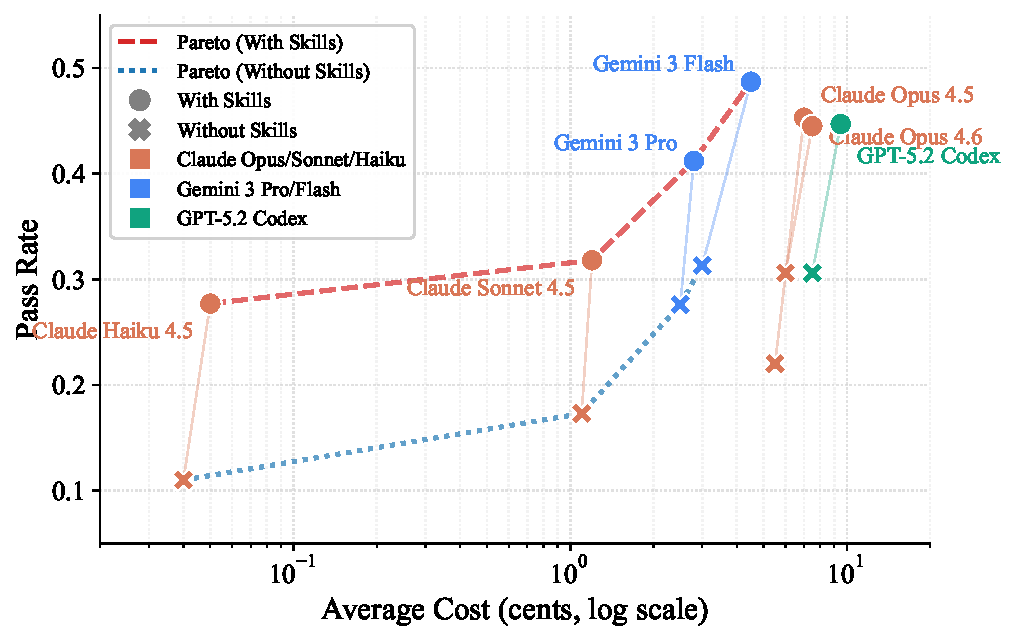
\includegraphics[width=\columnwidth]{figs/pareto_cost_vs_performance.pdf}
  % TODO: Regenerate Pareto figure with updated data
  \caption{Pareto frontier of pass rate vs.\ cost across model-harness configurations. Filled markers indicate with-Skills conditions; hollow markers indicate without-Skills. Skills shift the Pareto frontier upward, with Gemini~3 Flash and Claude~Opus dominating the with-Skills frontier. Cost positions in this figure reflect the evaluation infrastructure's pricing model. Trajectory analysis reveals that Flash consumes 2.3$\times$ more input tokens per task than Pro (1.08M vs.\ 0.47M), a compensatory strategy where the smaller model substitutes iterative exploration for reasoning depth. At official API pricing (\$0.50 vs.\ \$2.00 per 1M input tokens), Flash's 4$\times$ lower per-token cost more than offsets this higher volume, making Flash 44\% cheaper per task (\$0.55 vs.\ \$0.98).}
  \label{fig:pareto}
\end{figure}
\vspace{-10pt}

\subsubsection{Harness-Specific Reliability}

Beyond Skills efficacy, we observe reliability differences across commercial harnesses:

\begin{itemize}[nosep,leftmargin=*]
    \item \textbf{Claude Code}: Highest skills utilization rate; improvements range from +13.9pp (Opus 4.6) to +23.3pp (Opus 4.5), with all Claude models consistently benefiting.
    \item \textbf{Gemini CLI}: Highest raw performance (Gemini 3 Flash achieves 48.7\% with Skills); improvements range from +13.6pp to +17.4pp.
    \item \textbf{Codex CLI}: Competitive raw performance (44.7\% with Skills); frequently \emph{neglects} provided Skills---agents acknowledge Skills content but often implement solutions independently.
\end{itemize}
\vspace{-10pt}
\subsubsection{Domain-Level Analysis}


\begin{table}[h]
\vskip -0.05in
\centering
\small
\caption{Skills efficacy by domain across 84 evaluated tasks (11 domains). All domains show positive aggregate delta, though individual tasks within each domain may show negative effects.}
\label{tab:domain}
\resizebox{\columnwidth}{!}{
\begin{tabular}{lccc}
\toprule
\textbf{Domain} & \textbf{With Skills} & \textbf{No Skills} & \textbf{$\Delta_\text{abs}$} \\
\midrule
Healthcare & 86.1\% & 34.2\% & \ppos{51.9} \\
Manufacturing & 42.9\% & 1.0\% & \ppos{41.9} \\
Cybersecurity & 44.0\% & 20.8\% & \ppos{23.2} \\
Natural Science & 44.9\% & 23.1\% & \ppos{21.9} \\
Energy & 47.5\% & 29.5\% & \ppos{17.9} \\
Office \& White Collar & 42.5\% & 24.7\% & \ppos{17.8} \\
Finance & 27.6\% & 12.5\% & \ppos{15.1} \\
Media \& Content Production & 37.6\% & 23.8\% & \ppos{13.9} \\
Robotics & 27.0\% & 20.0\% & \ppos{7.0} \\
Mathematics & 47.3\% & 41.3\% & \ppos{6.0} \\
Software Engineering & 38.9\% & 34.4\% & \ppos{4.5} \\
\bottomrule
\end{tabular}
}
\vskip -0.05in
\end{table}

\paragraph{Finding 4: Skills benefit varies widely across domains.}
\autoref{tab:domain} presents Skill efficacy by domain, revealing substantial heterogeneity.
Healthcare (+51.9pp) and Manufacturing (+41.9pp) benefit most, while Mathematics (+6.0pp) and Software Engineering (+4.5pp) show smaller gains.
Domains requiring specialized procedural knowledge that is underrepresented in model pretraining (e.g., clinical data harmonization, manufacturing workflows) show the largest improvements, whereas domains with strong pretraining coverage benefit less from external procedural guidance.

\subsubsection{Task-Level Analysis}

Analysis of 84 individual tasks reveals high variance in Skills effectiveness:


\paragraph{Top Skills beneficiaries.} Tasks showing largest improvements: \nolinkurl{mario-coin-counting} (+85.7pp, from 2.9\% to 88.6\%), \nolinkurl{sales-pivot-analysis} (+85.7pp), \nolinkurl{flood-risk-analysis} (+77.1pp), \nolinkurl{sec-financial-report} (+74.3pp). These tasks involve specialized procedural knowledge rarely covered in pretraining.

\paragraph{Skills hurt performance on some tasks.} Despite positive domain-level aggregates, 16 of 84 tasks show negative Skills deltas: \nolinkurl{taxonomy-tree-merge} (--39.3pp), \nolinkurl{energy-ac-optimal-power-flow} (--14.3pp), \nolinkurl{trend-anomaly-causal-inference} (--12.9pp), \nolinkurl{exoplanet-detection-period} (--11.4pp). These failures suggest Skills may introduce conflicting guidance or unnecessary complexity for tasks models already handle well.

%==============================================================================
\subsection{Experiment 2: Skills Design Factors}
%==============================================================================

To understand \emph{how} Skills design affects efficacy, we analyze the relationship between Skills quantity, complexity, and performance.

\subsubsection{Skills Quantity Analysis}


\begin{table}[h]
\centering
\small
\caption{Pass rates by number of Skills provided. 2--3 Skills shows optimal benefit.}
\label{tab:skill-quantity}
\begin{tabular}{lccc}
\toprule
\textbf{Skills Count} & \textbf{With Skills} & \textbf{No Skills} & \textbf{$\Delta_\text{abs}$} \\
\midrule
1 skill & 42.2\% & 24.4\% & \ppos{17.8} \\
\textbf{2--3 skills} & \textbf{42.0\%} & \textbf{23.4\%} & \textbf{\ppos{18.6}} \\
4+ skills & 32.7\% & 26.9\% & \ppos{5.9} \\
\bottomrule
\end{tabular}
\end{table}

\paragraph{Finding 5: 2--3 Skills are optimal; more Skills show diminishing returns.}
\autoref{tab:skill-quantity} presents performance stratified by number of Skills provided per task.
Tasks with 2--3 Skills show the largest improvement (+18.6pp), while 4+ Skills provide only +5.9pp benefit. This non-monotonic relationship suggests that excessive Skills content creates cognitive overhead or conflicting guidance.

\subsubsection{Skills Complexity Analysis}


\begin{table}[h]
\centering
\small
\caption{Pass rates by Skills complexity level. Detailed and compact Skills outperform comprehensive ones.}
\label{tab:skill-complexity}
\begin{tabular}{lccc}
\toprule
\textbf{Complexity} & \textbf{Pass Rate} & \textbf{$\Delta_\text{abs}$} & \textbf{N} \\
\midrule
Detailed & 42.7\% & \ppos{18.8} & 1165 \\
Compact & 37.6\% & \ppos{17.1} & 845 \\
Standard & 37.1\% & \ppos{10.1} & 773 \\
Comprehensive & 39.9\% & \nneg{2.9} & 140 \\
\bottomrule
\end{tabular}
\end{table}

\paragraph{Finding 6: Moderate-length Skills outperform comprehensive ones.}
We present the effects of Skills documentation complexity on performance in \autoref{tab:skill-complexity}.
Detailed (+18.8pp) and compact (+17.1pp) Skills provide the largest benefit, while comprehensive Skills actually hurt performance (--2.9pp). This suggests that focused procedural guidance is more effective than exhaustive documentation---agents may struggle to extract relevant information from lengthy Skills content, and overly elaborate Skills can consume context budget without providing actionable guidance.

\subsubsection{Model Scale Effects}

We study the effects of the foundation models' scale across Claude model family (Opus, Sonnet, Haiku 4.5).
\vskip -1in
\paragraph{Finding 7: Smaller model + Skills can exceed larger model without Skills.} Claude Haiku 4.5 with Skills (27.7\%) outperforms Haiku without Skills (11.0\%) by +16.7pp. Meanwhile, Claude Opus 4.5 without Skills achieves 22.0\%. This demonstrates that Skills can partially compensate for model capacity limitations on procedural tasks.


